\subsection*{Træning} \label{sec:traening}
Når brugeren har angivet sin daglige helbredstilstand samt om der ønskes at tilkoble kompatible enheder til træningen, kan denne begyndes. Aktivitetsdiagrammet over træningen fremgår af \autoref{fig:traening}. 

\begin{figure} [H]
\centering
\textbf{Aktivitetsdiagram: Træning}\par\medskip
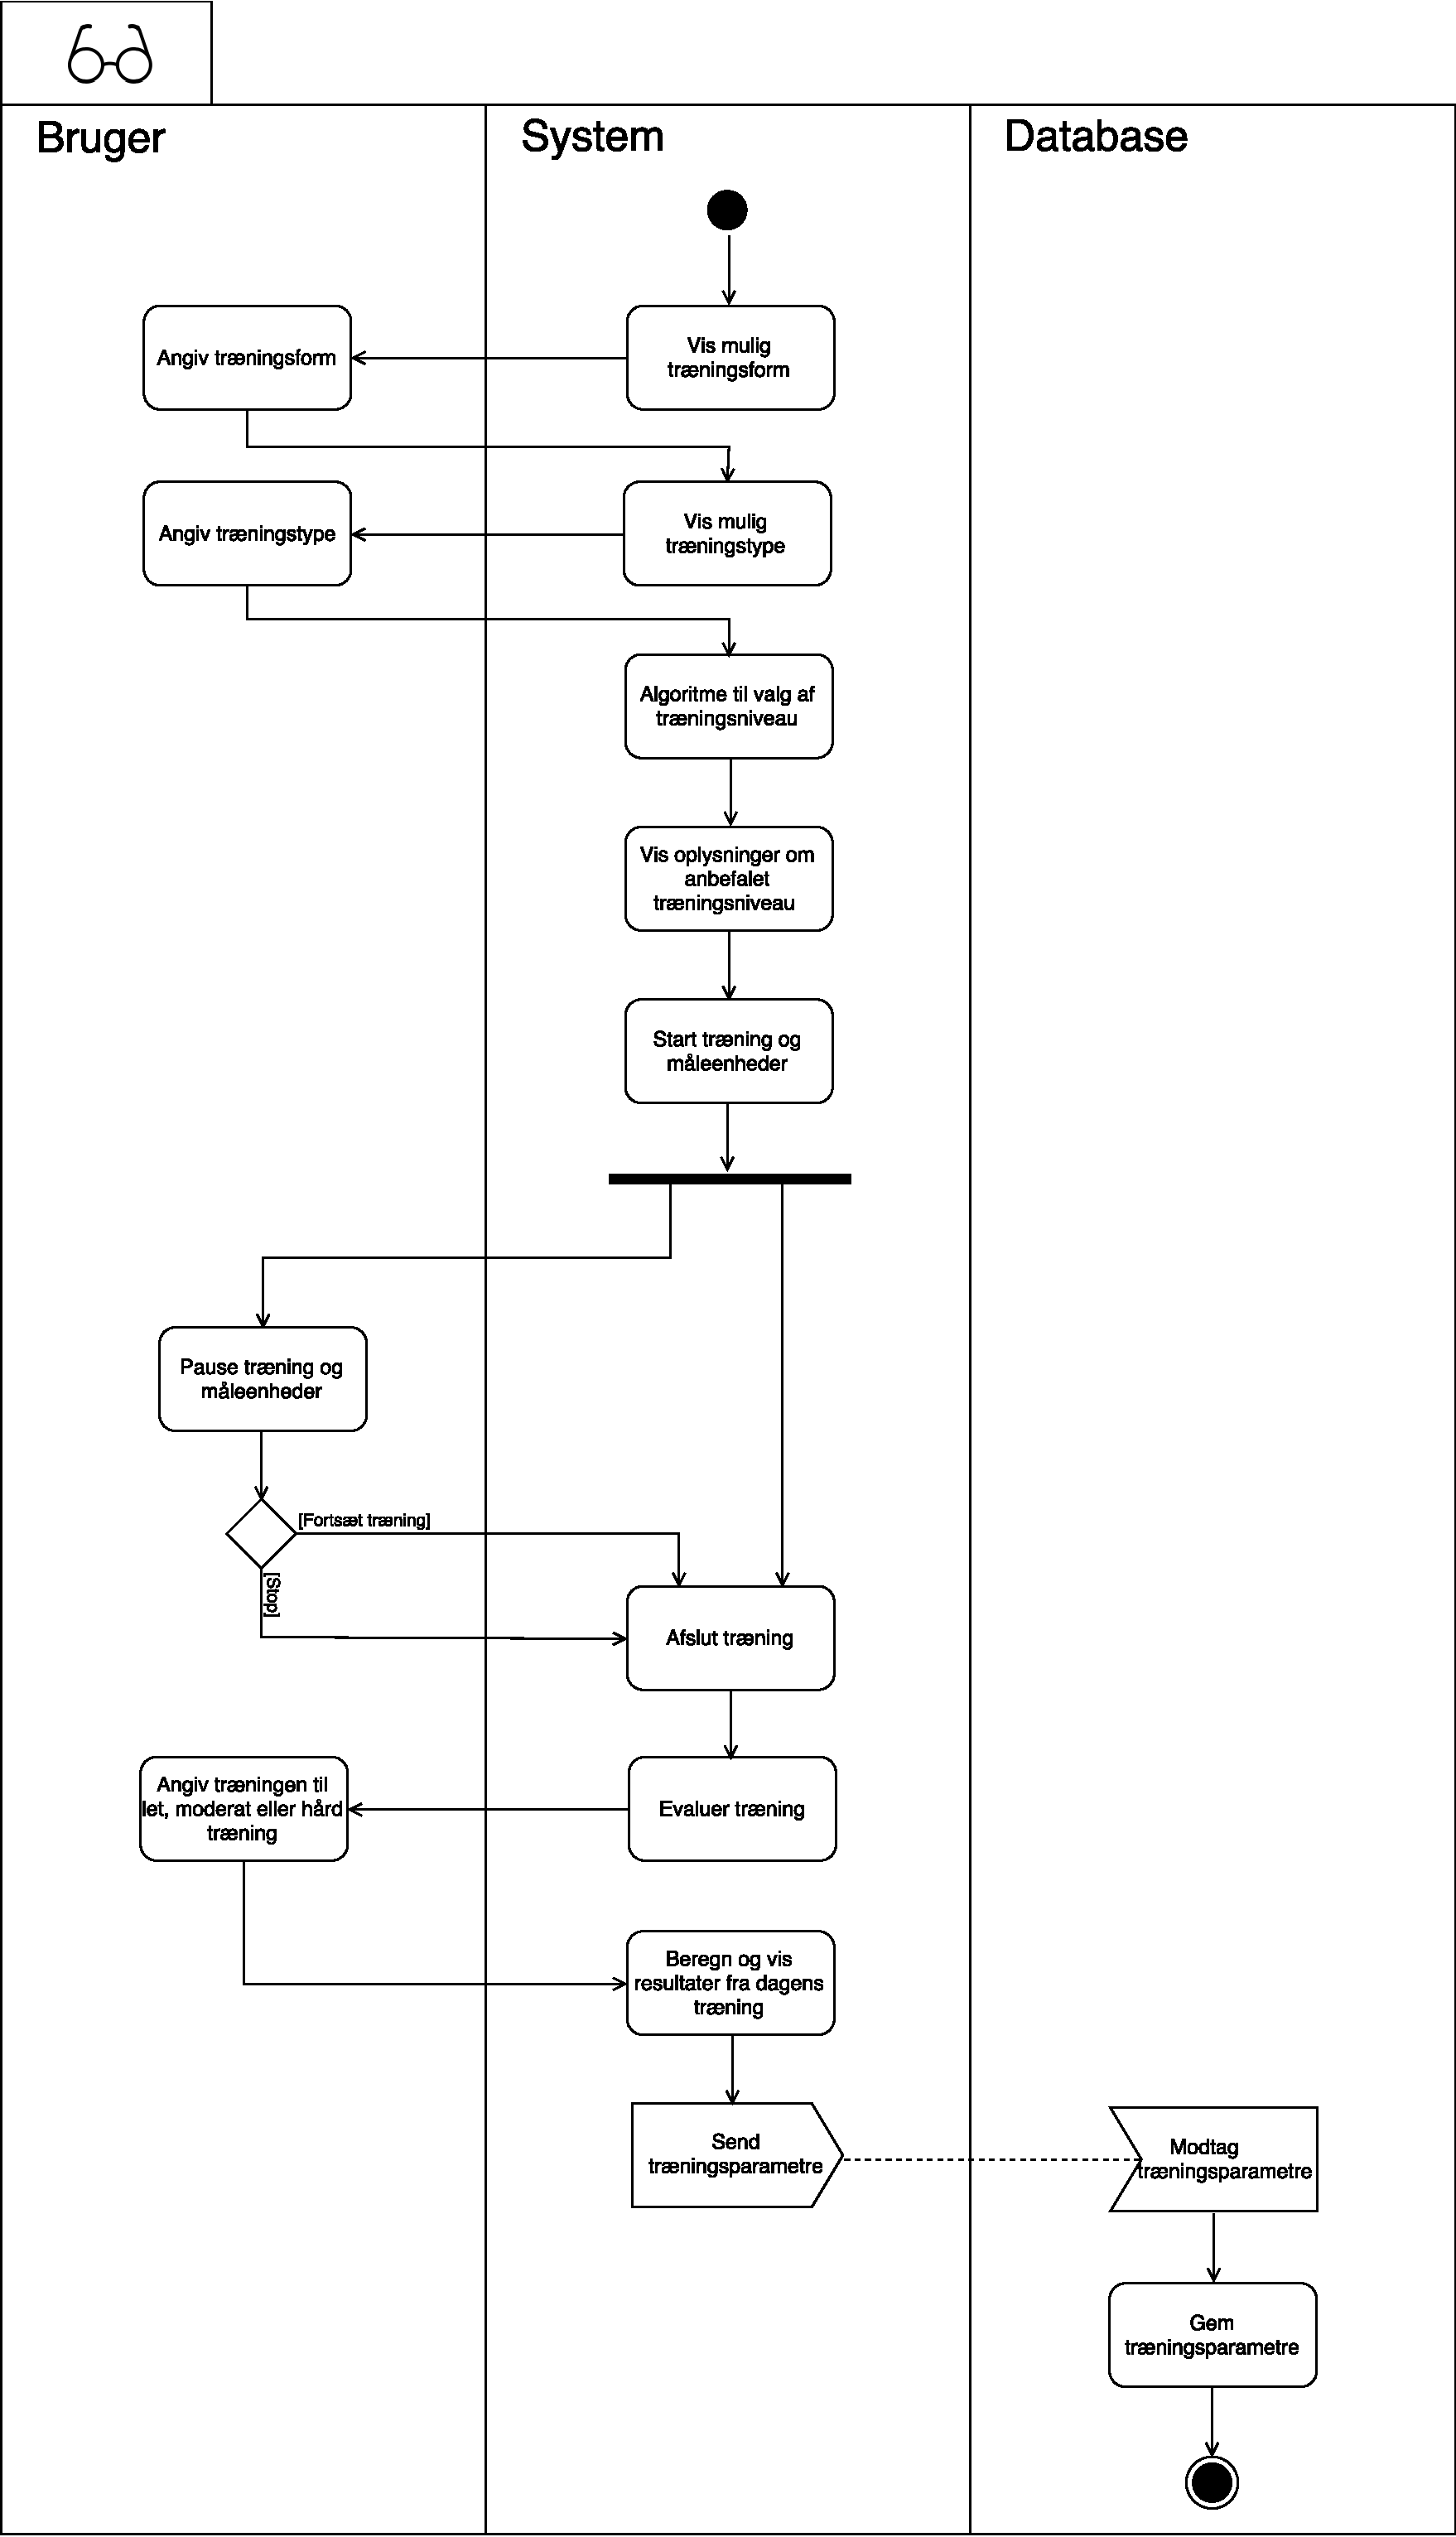
\includegraphics[width=0.8\textwidth]{figures/aktivitetsdiagram/NYTraening}
\caption{Aktivitetsdiagram over træning.}
\label{fig:traening}
\end{figure}

\noindent
Før selve træningen kan påbegyndes, skal brugeren angive træningsform, herunder konditions-, styrketræning og vejrtrækningsøvelser. Ud fra den valgte træningsform skal brugeren angive træningstype f.eks. gå, løbe eller cykle. Efterfølgende beregnes et anbefalet træningsniveau ud fra en algoritme på baggrund af kategoriseringen af KOL, den daglige helbredstilstand samt evalueringer fra forhenværende træning. Oplysninger om det anbefalede træningsniveau vises og træningen samt måleenheder kan påbegyndes. 

Under træningen kan brugeren pause træningen og måleenhederne, hvorefter der er mulighed for at fortsætte træningen eller afslutte træningen. Afsluttes eller fuldføres træningen, skal brugere evaluere træningen. Denne evalueres som let, moderat eller hård. Herefter vises resultater fra den udførte træning. Systemet sender træningsparametre, som består af den daglige helbredstilstand, resultater fra den udførte træning samt evaluering til databasen, som lagrer informationerne. 
